%chapter 1
\chapter{Transportation System}
%
\section{Introduction}
Transportation is a crucial aspect of a nation's development and prosperity. However, with the advent of modern means of transportation, managing its operation has become more complex, so there is ample opportunity for engineers to devise new operational and management techniques for the smooth control of various modes of transportation of a country. 

\section{History of Transportation}
\subsection*{Early Boats}
\par
The first mode of transportation was created in the effort to traverse water: boats. Those who colonized Australia roughly 60,000–40,000 years ago have been credited as the first people to cross the sea, though there is some evidence that seafaring trips were carried out as far back as 900,000 years ago.
\par
The earliest known boats were simple logboats, also referred to as dugouts, which were made by hollowing out a tree trunk. Evidence for these floating vehicles comes from artifacts that date back to around 10,000–7,000 years ago. The Pesse canoe—a logboat—is the oldest boat unearthed and dates as far back as 7600 BCE. Rafts have been around nearly as long, with artifacts showing them in use for at least 8,000 years.
\subsection*{Horses and Wheeled Vehicles}
\par
Next, came horses. While it’s difficult to pinpoint exactly when humans first began domesticating them as a means of getting around and transporting goods, experts generally go by the emergence of certain human biological and cultural markers that indicate when such practices started to take place.
\par
Based on changes in teeth records, butchering activities, shifts in settlement patterns, and historic depictions, experts believe that domestication took place around 4000 BCE. Genetic evidence from horses, including changes in musculature and cognitive function, support this.
\par
It was also roughly around this period that the wheel was invented. Archaeological records show that the first wheeled vehicles were in use around 3500 BCE, with evidence of the existence of such contraptions found in Mesopotamia, the Northern Caucuses, and Central Europe. The earliest well-dated artifact from that time period is the "Bronocice pot," a ceramic vase that depicts a four-wheeled wagon that featured two axles. It was unearthed in southern Poland.
\\
\subsection*{Steam Engines}
\par
In 1769, the Watt steam engine changed everything. Boats were among the first to take advantage of steam-generated power; in 1783, a French inventor by the name of Claude de Jouffroy built the "Pyroscaphe," the world’s first steamship. But despite successfully making trips up and down the river and carrying passengers as part of a demonstration, there wasn’t enough interest to fund further development.
\par
While other inventors tried to make steamships that were practical enough for mass transport, it was American Robert Fulton who furthered the technology to where it was commercially viable. In 1807, the Clermont completed a 150-mile trip from New York City to Albany that took 32 hours, with the average speed clocking in at about five miles per hour. Within a few years, Fulton and company would offer regular passenger and freight service between New Orleans, Louisiana, and Natchez, Mississippi.
\par
Back in 1769, another Frenchman named Nicolas Joseph Cugnot attempted to adapt steam engine technology to a road vehicle—the result was the invention of the first automobile. However, the heavy engine added so much weight to the vehicle that it wasn't practical. It had a top speed of 2.5 miles per hour.
\par
Another effort to repurpose the steam engine for a different means of personal transport resulted in the "Roper Steam Velocipede." Developed in 1867, the two-wheeled steam-powered bicycle is considered by many historians to be the world’s first motorcycle.
\\
\subsection*{Locomotives}
\par
One mode of land transport powered by a steam engine that did go mainstream was the locomotive. In 1801, British inventor Richard Trevithick unveiled the world’s first road locomotive—called the “Puffing Devil”—and used it to give six passengers a ride to a nearby village. It was three years later that Trevithick first demonstrated a locomotive that ran on rails, and another one that hauled 10 tons of iron to the community of Penydarren, Wales, to a small village called Abercynon.
\par
It took a fellow Brit—a civil and mechanical engineer named George Stephenson—to turn locomotives into a form of mass transport. In 1812, Matthew Murray of Holbeck designed and built the first commercially successful steam locomotive, “The Salamanca,” and Stephenson wanted to take the technology a step further. So in 1814, Stephenson designed the "Blücher," an eight-wagon locomotive capable of hauling 30 tons of coal uphill at a speed of four miles per hour.
\par
By 1824, Stephenson improved the efficiency of his locomotive designs to where he was commissioned by the Stockton and Darlington Railway to build the first steam locomotive to carry passengers on a public rail line, the aptly named "Locomotion No. 1." Six years later, he opened the Liverpool and Manchester Railway, the first public inter-city railway line serviced by steam locomotives. His notable accomplishments also include establishing the standard for rail spacing for most of the railways in use today. No wonder he’s been hailed as "Father of Railways."
\\
\subsection*{Submarines}
\par
Technically speaking, the first navigable submarine was invented in 1620 by Dutchman Cornelis Drebbel. Built for the English Royal Navy, Drebbel’s submarine could stay submerged for up to three hours and was propelled by oars. However, the submarine was never used in combat, and it wasn’t until the turn of the 20th century that designs leading to practical and widely used submersible vehicles were realized.
\par
Along the way, there were important milestones such as the launch of the hand-powered, egg-shaped "Turtle" in 1776, the first military submarine used in combat. There was also the French Navy submarine "Plongeur," the first mechanically powered submarine.
\par
Finally, in 1888, the Spanish Navy launched the "Peral," the first electric, battery-powered submarine, which also so happened to be the first fully capable military submarine. Built by a Spanish engineer and sailor named Isaac Peral, it was equipped with a torpedo tube, two torpedoes, an air regeneration system, and the first fully reliable underwater navigation system, and it posted an underwater speed of 3.5 miles per hour.
\\
\subsection*{Aircraft}
\par
The start of the twentieth century was truly the dawn of a new era in the history of transportation as two American brothers, Orville and Wilbur Wright, pulled off the first official powered flight in 1903. In essence, they invented the world’s first airplane. Transport via aircraft took off from there with airplanes being put into service within a few short years during World War I. In 1919, British aviators John Alcock and Arthur Brown completed the first transatlantic flight, crossing from Canada to Ireland. The same year, passengers were able to fly internationally for the first time.
\par
Around the same time that the Wright brothers were taking flight, French inventor Paul Cornu started developing a rotorcraft. And on November 13, 1907, his "Cornu" helicopter, made of little more than some tubing, an engine, and rotary wings, achieved a lift height of about one foot while staying airborne for about 20 seconds. With that, Cornu would lay claim to having piloted the first helicopter flight.
\\\\
\section{Transportation Sector and Modes of Transportation}
\subsection{Transportation Sector}
\par
Transportation sector performs transportation services in order to satisfy demand for mobility of people and transport of freight shipments.A range of socioeconomic activities in a society, as well as land uses induce transportation demand. The demand is represented by the number of passengers and/or volumes of cargo to be transported between given origins and destinations during a given (specified) period of time. The supply component in the transportation sector consists of transport services provided by different transport modes and their particular systems. Airports, highways, streets, and ports should be able to meet transportation demand and offer acceptable level-of-service to the users. The transport supply component contributes to the economy of a region, country, and continent it serves. The demand and supply component are in permanent interaction.
\subsection{Modes of Transportation}
\par
The transportation modes constituting the supply component are generally classified according to
the way of performing their operations of transporting people and freight shipments. In general, the basic land-based transport modes include road, rail, and pipeline. The water-based mode includes inland waterways and sea shipping. The air transport is the air-based mode. The specific mode is intermodal transport consisting of combinations of particular basic modes and their systems. In addition, the mode not carrying out physical entities but just information is telecommunications. Fig. shows a simplified scheme of the structure of transport sector, its modes and their systems.
\\\\
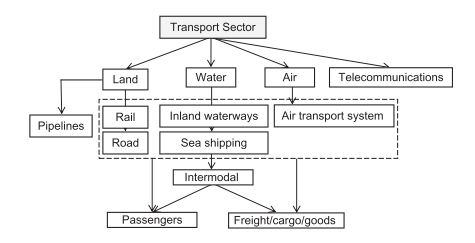
\includegraphics{gfx/fig1.png}
\par
Transport modes generally consist of two types of systems: the first is intended for serving passenger and the other for serving freight/cargo/goods demand. Each of these consists of subsystems, which will be called systems. The classification of systems within each mode is carried out at three levels: (i) type of the system (passengers, freight), spatial scale of operation (urban/suburban/regional, interurban), and carrier type (individual, group).
\\\\
The Fig. below shows classification of systems of the road transport mode.
\\\\
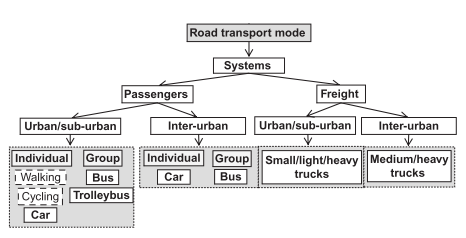
\includegraphics{gfx/fig2.png}
\\\\
%
\section{Factors influencing Transport Operations}
\par
There are mainly four components of road transportation: the driver, the pedestrian, the vehicle, and the road, which influence road transport management's design and operational considerations. To provide efficient and safe road transportation, a knowledge of the characteristics and limitations of each of these components is essential. It is also crucial to be aware of the interrelationships among these components to determine the effects they have on each other. Their characteristics are also of primary importance when traffic engineering measures such as traffic control devices are used in the highway mode.
\subsection{Driver Characteristics}
\par
One problem that faces traffic and transportation engineers when they consider driver characteristics in the course of design is the varying skills and perceptual abilities of drivers on the highway, demonstrated by a wide range of capabilities to hear, see, evaluate, and react to information. Studies support that these abilities vary under different conditions, such as the influence of alcohol, fatigue, and time of the day. Therefore, it is essential that criteria used for design purposes be compatible with the capabilities and limitations of most drivers on the highway. The use of an average value, such as mean reaction time, may not be adequate for a large number of drivers. The 85th percentile and the 95th percentile have been used to select design criteria; in general, the higher the chosen percentile, the wider the range covered.
\subsubsection{The Human Response Process}
Actions taken by the drivers while driving result from their evaluation and reaction to the information they obtain from their certain stimuli. However, assessment and response must be carried out quickly, as the information received while driving the highways is dynamic. Furthermore, it has been suggested that most of the information received by a driver is visual, implying that the ability to see is of fundamental importance in the driving task. Therefore, highway and traffic engineers must have some rudimentary knowledge of visual perception and hearing perception.
%
\paragraph{Visual Reception}: The principal characteristics of the eye are visual acuity, peripheral vision, color vision, glare vision and recovery, and depth perception.
%
\subparagraph{1. Visual Acuity}: It is the ability to see fine details of an object. It can be represented by the visual angle, which is the reciprocal of the smallest pattern detail in minutes of arc that can be resolved and given as:
\\\\
\begin{equation}
	\phi = 2 \arctan\left(\frac{L}{2D}\right)
\end{equation}
Where,
\\
\hspace*{10mm}L = diameter of the target (letter or symbol)
\\
\hspace*{10mm}D = distance from the eye to target in the same units as L
\\\\
Mathematical Derivation,
\\
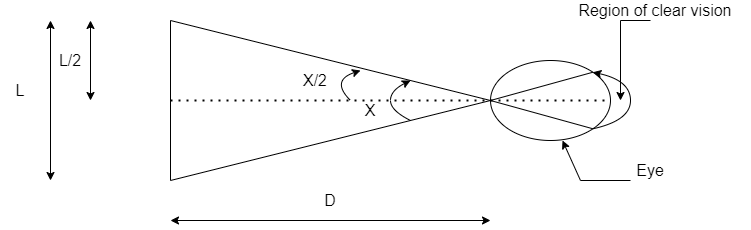
\includegraphics[scale= 0.5]{gfx/fig3.png}
\\
Using trigonometry,
\\
\begin{gather*}
	\tan\left(\frac{X}{2}\right) = \frac{\frac{L}{2}}{D}\\
	\tan\left(\frac{X}{2}\right) = \frac{L}{2D}\\
	 X = 2 \arctan\left(\frac{L}{2D}\right)
\end{gather*}
\\\\
The ability to resolve a pattern detail with a visual acuity of one minute of arc (1/60 of a degree) is considered as normal vision of acuity (20/20 vision).
\\\\
\begin{itshape}
	*20/20 vision is a term used to express normal visual acuity measured at a distance of 20 feet. If you have 20/20 vision, you can see clearly at 20 ft what should normally be seen at that distance. If you have 20/100 vision, it means you must be as close as 20ft to see what a person with normal vision can see at 100ft.
\end{itshape}
\\
\subparagraph{2. Peripheral Vision}: It is the ability of people to see objects beyond the cone of clearest vision. Although objects can be seen within this zone, details and color are not clear. The cone for peripheral vision could be one subtending up to 160 degrees; this value is affected by the speed of the vehicle. Age also influences peripheral vision. For instance, at about age 60, a significant change occurs in a person’s peripheral vision.
\\
\subparagraph{3. Color Vision}: It is the ability to differentiate one color from another, but deficiency in this ability, usually referred to as color blindness, is not of great significance in highway driving because other ways of recognizing traffic information devices (e.g., shape) can compensate for it. Combinations of black and white and black and yellow have been shown to be those to which the eye is most sensitive.
\\
\subparagraph{4. Glare Vision and Recovery}: There are two types of glare vision: direct and specular. Rowland and others have indicated that direct glare occurs when relatively bright light appears in the individual’s field of vision and specular glare occurs when the image reflected by the relatively bright light appears in the field of vision. Both types of glare result in a decrease of visibility and cause discomfort to the eyes. It is also known that age has a significant effect on the sensitivity to glare, and that at about age 40, a significant change occurs in a person’s sensitivity to glare.\par
The time required by a person to recover from the effects of glare after passing the light source is known as glare recovery. Studies have shown that this time is about 3 seconds when moving from dark to light and can be 6 seconds or more when moving from light to dark. Glare vision is of great importance during night driving; it contributes to the problem of serving older people, who see much more poorly at night. This phenomenon should be taken into account in the design and location of street lighting so that glare effects are reduced to a minimum.\par
Glare effects can be minimized by reducing luminaire brightness and by increasing the background brightness in a driver’s field of view. Specific actions taken to achieve this in lighting design include using higher mounting heights, positioning lighting supports farther away from the highway, and restricting the light from the luminaire to obtain minimum interference with the visibility of the driver.
\\
\subparagraph{5. Depth Perception}: It affects the ability of a person to estimate speed and distance. It is particularly important on two-lane highways during passing maneuvers, when head-on crashes may result from a lack of proper judgment of speed and distance.\par
The ability of the human eye to differentiate between objects is fundamental to this phenomenon. It should be noted, however, that the human eye is not very good at estimating absolute values of speed, distance, size, and acceleration. This is why traffic control devices are standard in size, shape, and color. Standardization not only aids in distance estimation but also helps the color-blind driver to identify signs.
\\
\subsubsection{Perception-Reaction Process}
The process through which a driver, cyclist, or pedestrian evaluates and reacts to a stimulus can be divided into four subprocesses:
\begin{enumerate}
	\item \emph{Perception:} the driver sees a control device, warning sign, or object on the road
	\item \emph{Identification:} the driver identifies the object or control device and thus understands the stimulus
	\item \emph{Emotion:} the driver decides what action to take in response to the stimulus; for example, to step on the brake pedal, to pass, to swerve, or to change lanes
	\item \emph{Reaction or Volition:} the driver actually executes the action decided on during the emotion sub-process
\end{enumerate}
\par
Time elapses during each of these subprocesses. The time that elapses from the start of perception to the end of reaction is the total time required for perception, identification, emotion, and volition, sometimes referred to as PIEV time or (more commonly) as perception-reaction time.\\
\par
Perception-reaction time is an important factor in the determination of braking distances, which in turn dictates the minimum sight distance required on a highway and the length of the yellow phase at a signalized intersection. Perception-reaction time varies among individuals and may, in fact, vary for the same person as the occasion changes. These changes in perception-reaction time depend on how complicated the situation is, the existing environmental conditions, age, whether the person is tired or under the influence of drugs and/or alcohol, and whether the stimulus is expected or unexpected.\\
\par
Triggs and Harris described this phenomenon in detail. They noted that the 85th-percentile time to brake, obtained from several situations, varied from 1.26 to over 3 seconds. The reaction time selected for design purposes should, however, be large enough to include reaction times for most drivers using the highways. Recommendations made by the American Association of State Highway and Transportation Officials (AASHTO) stipulate 2.5 seconds for stopping-sight distances. This encompasses the decision times for about 90 percent of drivers under most highway conditions. Note, however, that a reaction time of 2.5 second may not be adequate for unexpected conditions or for some very complex conditions, such as those at multiphase at-grade intersections and ramp terminals. For example, when signals are unexpected, reaction times can increase by 35 percent.
\\\\
\emph{Numerical Example:}
\\
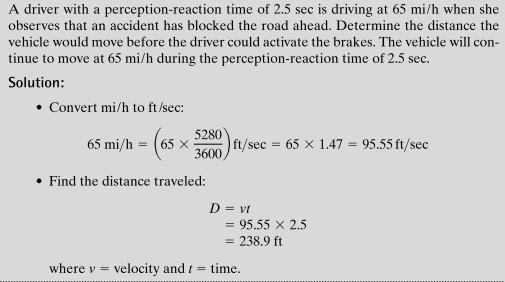
\includegraphics{gfx/fig4.png}
\\\\
\subsection{Vehicle Characteristics}
Criteria for the geometric design of highways are partly based on the static, kinematic, and dynamic characteristics of vehicles. Static characteristics include the weight and size of the vehicle, while kinematic characteristics involve the motion of the vehicle without considering the forces that cause the motion. Dynamic characteristics involve the forces that cause the motion of the vehicle. Since nearly all highways carry both passenger-automobile and truck traffic, it is essential that design criteria take into account the characteristics of different types of vehicles. A thorough knowledge of these characteristics will aid the highway and/or traffic engineer in designing highways and traffic-control systems that allow the safe and smooth operation of a moving vehicle, particularly during the basic maneuvers of passing, stopping, and turning. Therefore, designing a highway involves the selection of a design vehicle, whose characteristics will encompass those of nearly all vehicles expected to use the highway. The characteristics of the design vehicle are then used to determine criteria for geometric design, intersection design, and sight-distance requirements.

\subsubsection{Static characteristics}
The size of the design vehicle for a highway is an important factor in the determination of design standards for several physical components of the highway. These include lane width, shoulder width, length and width of parking bays, and lengths of vertical curves. The axle weights of the vehicles expected on the highway are important when pavement depths and maximum grades are being determined.\\
\par
For many years, each state prescribed by law the size and weight limits for trucks using its highways, and in some cases local authorities also imposed more severe restrictions on some roads. Table 3.1 shows some features of static characteristics for which limits were prescribed. A range of maximum allowable values is given for each feature.
\\\\
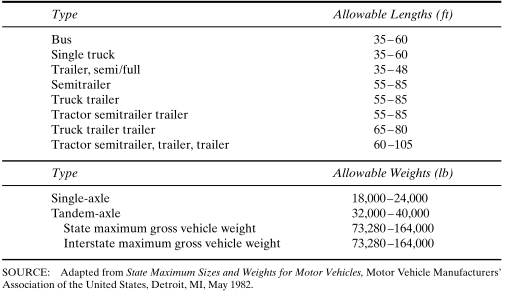
\includegraphics{gfx/fig5.png}
\emph{Fig: Range of State Limits on Vehicle Lengths by Type and Maximum Weight of Vehicle}
\\\\
Since the passage of the Surface Transportation Assistance Act of 1982, the maximum allowable truck sizes and weights on Interstate and other qualifying federal-aided highways are at most:
\begin{itemize}
	\item 80,000 lb gross weight, with axle loads of up to 20,000 lb for single axles and 34,000 lb for tandem (double) axles
	\item 102 in. width for all trucks
	\item 48 ft length for semitrailers and trailers
	\item 28 ft length for each twin trailer
\end{itemize}
%
(Note: Those states that had higher weight limits before this law was enacted are allowed to retain them for intrastate travel.)
\\\\
\par
The federal regulations also stipulate that the overall maximum gross weight for a group of two or more consecutive axles should be determined from the equation:
\begin{equation}
	W = 500\left[\frac{LN}{N-1} + 12N + 36\right]
\end{equation}
Where,\\
\hspace*{10mm}W = overall gross weight (calculated to the nearest 500 lb)\\
\hspace*{10mm}L = the extreme of any group of two or more consecutive axles (ft)\\
\hspace*{10mm}N = number of axles in the group under consideration\\\\
%
The regulations also stipulate that a gross load of 34,000 lb may be carried by two consecutive sets of tandem axles if the overall distance between the first and last axles of the consecutive sets is 36 ft or more.
\\\\
\emph{Numerical Example:}
\\
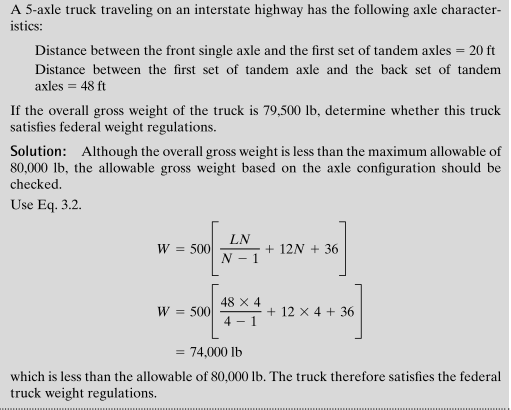
\includegraphics{gfx/fig6.png}
\newpage
Because the static characteristics of the predominant vehicles are used to
establish certain geometric parameters of the road, vehicles have been classified so that they represent static characteristics within a particular class. AASHTO has classified automobiles into four general classes of vehicles: passenger cars, buses, trucks, and recreational vehicles. Vehicles included in the passenger-car class are all sizes of passenger cars, sport/utility vehicles, minivans, vans, and pick-up trucks. Those in the bus class include intercity (motor coaches), city transit, school, and articulated buses. Vehicles in the truck class are single-unit trucks, truck tractor–semitrailer combinations, and trucks or truck tractors with semitrailers in combination with full trailers. Vehicles in the recreational-vehicle class are motor homes, cars with camper trailers, cars with boat trailers, motor homes with boat trailers, and motor homes pulling cars. The largest and most frequent vehicle expected to use the facility is selected as the design vehicle, and the following
guidelines are provided for selection:
\begin{enumerate}
	\item For parking lots or a series of parking lots, passenger-car class could be considered.
	\item For intersections on residential streets and park roads, a single-unit truck class could be considered.
	\item For intersections of state highways with city streets on which buses travel, but on which relatively few large trucks travel, a city transit bus class could be considered.
	\item For intersections of highways with low-volume county highways and
	township/local roads with traffic volume under 400 Average Daily Traffic
	(ADT), a large school bus (84 passengers) or a conventional school bus
	(65 passengers) could be considered.
	\item For other intersections of state highways and industrial streets with high volumes of traffic and/or providing large truck access to local facilities, the minimum design vehicle is the WB20 (WB65 or WB67) 
	\item For intersections of freeway ramp terminals with arterial crossroads the minimum design vehicle is the WB20 (WB65 or WB67)
\end{enumerate}
The characteristic of vehicle categories that influence design of intersections
when speeds are 15 km/h or less are (1) the minimum centerline radius (CTR);
(2) the out-to-out track width; (3) the wheel base; and (4) the path of the inner
rear tire of the vehicle as it makes a turn at the intersection. When turns are
made at speeds of 10 km/h or less, the turning radius and turning path depend
mainly on the size of the vehicle making the turn. These have therefore been
established for each design vehicle.
\newpage
\begin{center}
	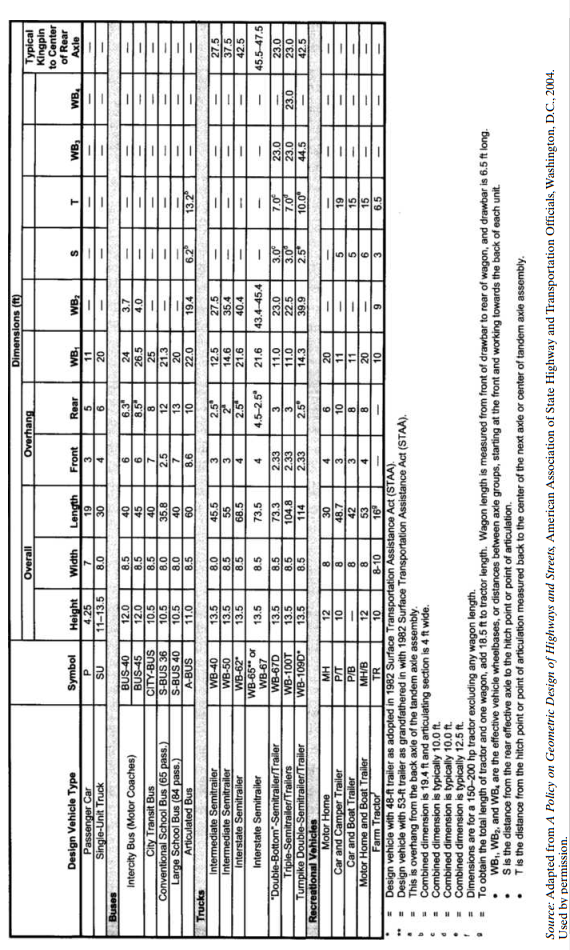
\includegraphics[scale=0.8]{gfx/staticDesignTable.png}
\end{center} 
\newpage
\subsubsection{Kinematic Characteristics}
The primary element among kinematic characteristics is the acceleration capability of the vehicle. Acceleration capability is important in several traffic operations, such as passing maneuvers and gap acceptance. Also, the dimensioning of highway features such as freeway ramps and passing lanes is often governed by acceleration rates. Acceleration is also important in determining the forces that cause motion. Therefore, a study of the kinematic characteristics of the vehicle primarily involves a study of how acceleration rates influence the elements of motion, such as velocity and distance. We therefore review in this section the mathematical relationships among acceleration, velocity, distance, and time.
\\\\
Let us consider a vehicle moving along a straight line from point o to point m, a distance x in a reference plane T. The position vector of the vehicle after time t may be expressed as:
\begin{equation}
	r_{om} = x \hat{i}
\end{equation}
\\
Where,\\
\hspace*{10mm}$ r_{om} $ = positon vector for m in T\\
\hspace*{10mm}$\hat{i}$ = a unit vector parallel to line om\\
\hspace*{10mm}$x$ = distance along the straight line\\\\
The velocity and acceleration for m may be simply expressed as
\begin{gather}
	u_m = \dot{r}_{om} = \dot{x}_{\hat{i}}\\
	a_m = \ddot{r}_{om} = \ddot{x}_{\hat{i}}
\end{gather}
\\
Where,\\
\hspace*{10mm}$u_m$ = velocity of the vehicle at point m\\
\hspace*{10mm}$a_m$ = accleration of the vehicle at point m\\
\hspace*{10mm}$\dot{x} = \frac{dy}{dx}$\\
\hspace*{10mm}$\ddot{x} = \frac{d^2y}{dx^2}$\\
\par
Two cases are of interest: (1) acceleration is assumed constant; (2) acceleration is a function of velocity.
\paragraph{Case 1: Acceleration is constant}
When the acceleration of the vehicle is assumed to be constant,
\begin{gather}
	\ddot{x}_{\hat{i}} = a\\
	\frac{d\dot{x}}{dt} = a\\
	\dot{x} = a t + C_1\\
	x =\frac{1}{2}a t^2 + C_1t+ C_2
\end{gather}
The constants $C_1$ and $C_2$ are determined either by the initial conditions on velocity and position or by using known positions of the vehicle at two different times.
\paragraph{Case 2: Acceleration is the function of velocity}
The assumption of constant acceleration has some limitations, because the accelerating capability of a vehicle at any time t is related to the speed of the vehicle at that time $(u_t)$. The lower the speed, the higher the acceleration rate that can be obtained. One model that is used commonly in this case is\\
\begin{equation}
	\label{case2}
	\frac{du_t}{dt} = \alpha - \beta u_t
\end{equation}
Where $\alpha$ and $\beta$ are constants.\\\\
In this model, the maximum acceleration rate that can be achieved is theoretically $\alpha$, which means that $\alpha$ has units of acceleration as its unit. The term $\beta u_t$ also should have units of acceleration as its unit, which means that b has the inverse of time (for example, $sec^-1$) as its unit.\\\\
Integrating Equation \ref{case2} gives,
\begin{equation*}
	-\frac{1}{\beta}\ln (\alpha - \beta u_t) = t + C
\end{equation*}
If the velocity is $u_o$ at $t = 0$,
\begin{gather*}
	C = -\frac{1}{\beta}\ln (\alpha - \beta u_o)\\
	-\frac{1}{\beta}\ln (\alpha - \beta u_t) = t  -\frac{1}{\beta}\ln (\alpha - \beta u_o)\\
	\ln\frac{(\alpha - \beta u_o)}{(\alpha - \beta u_t)} = \beta t\\
\end{gather*}
\begin{equation}
	\therefore t = \frac{1}{\beta}\ln\frac{(\alpha - \beta u_o)}{(\alpha - \beta u_t)}
\end{equation}
\begin{equation*}
	\alpha - \beta u_t = (\alpha - \beta u_o) e^{-\beta t}
\end{equation*}
\begin{equation}
	\label{acln}
	u_t = \frac{\alpha}{\beta} (1 - e^{-\beta t}) + u_o e^{-\beta t}
\end{equation}
The distance $x(t)$ traveled at any time $t$ may be determined by integrating equation \ref{acln}
\begin{gather*}
	x = \int_0^t u_t dt = \int_0^t \left[\frac{\alpha}{\beta} (1 - e^{-\beta t}) + u_o e^{-\beta t} \right] dt\\
	= \left[ \frac{\alpha}{\beta} \left( t + \frac{e^{-\beta t}}{\beta} \right) - \frac{u_o}{\beta} e^{\beta t} \right]_0^t\\
	= \left[ \frac{\alpha}{\beta}  t + \frac{\alpha}{\beta^2} e^{- \beta t} - \frac{u_o}{\beta} e^{- \beta t} \right]\\
	= \frac{\alpha}{\beta} t + \frac{\alpha}{\beta^2} e^{-\beta t} - \frac{u_o}{\beta} e^{-\beta t} - \frac{\alpha}{\beta^2} + \frac{u_0}{\beta}\\
	= \left(\frac{\alpha}{\beta}\right)t - \frac{\alpha}{\beta^2}(1 - e^{-\beta t}) + \frac{u_o}{\beta}(1 - e^{-\beta t})
\end{gather*}\\\\
\newpage
\emph{Numerical Example:}\\
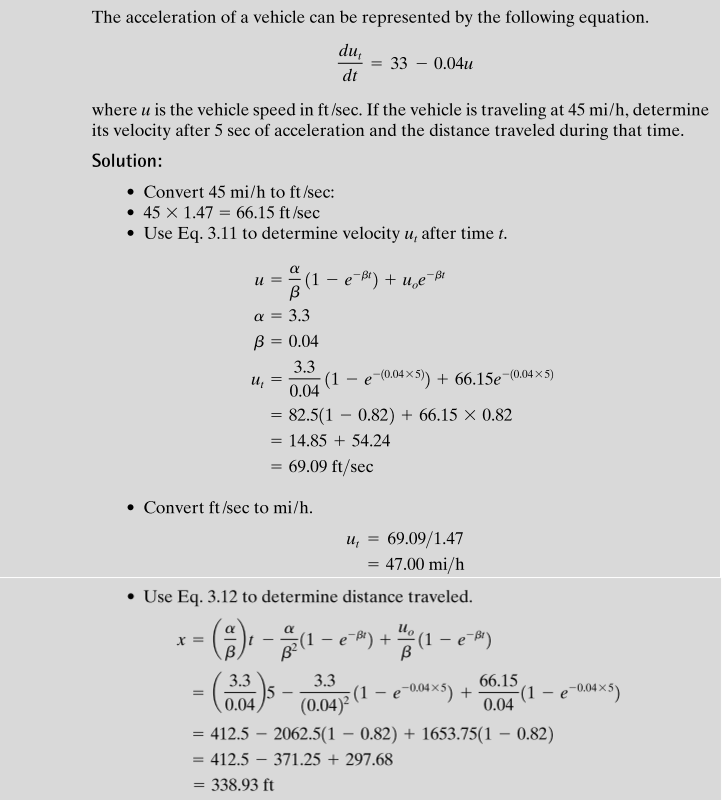
\includegraphics[scale=0.5]{gfx/fig7.png}
\subsubsection{Dynamic Characteristics}
Several forces act on a vehicle while it is in motion: air resistance, grade resistance, rolling resistance, and curve resistance. The extents to which these forces affect the operation of the vehicle are discussed in this section.
\paragraph{Air Resistance}
A vehicle in motion has to overcome the resistance of the air in front of it as well as the force due to the frictional action of the air around it. The force required to overcome these is known as the air resistance and is related to the cross-sectional area of the vehicle in a direction perpendicular to the direction of motion and to the square of the speed of the vehicle. Claffey has shown that this force can be estimated from the formula
\begin{equation}
	R_a = \frac{1}{2}\frac{(2.15\rho C_d A u^2)}{g}
\end{equation}
Where,\\
\hspace*{10mm}$R_a$ = air resistance force (lb)\\
\hspace*{10mm}$\rho$ = density of air (0.0766 $ lb/ft^3 $) at sea level; less at higher elevations\\
\hspace*{10mm}$C_d$ = aerodynamic drag coefficient\\
\hspace*{10mm}(current average value for passenger cars is 0.4; for trucks, this value ranges from 0.5 to 0.8, but a typical value is 0.5)\\
\hspace*{10mm}$A$ = frontal cross-sectional area ($ ft^2 $)\\
\hspace*{10mm}$u$ = vehicle speed (mi/h)\\
\hspace*{10mm}$g$ = acceleration of gravity (32.2 ft /sec2)\\\\
\begin{equation}
	R_a = \frac{0.0772 \times \rho \times C_D \times A \times u^2}{2}
\end{equation}
Where,\\
\hspace*{10mm}$R_a$ = air resistance force (N)\\
\hspace*{10mm}$\rho$ = density of air (1.227 $ kg/m^3 $) at sea level; less at higher elevations\\
\hspace*{10mm}$C_d$ = aerodynamic drag coefficient\\
\hspace*{10mm}(current average value for passenger cars is 0.4; for trucks, this value ranges from 0.5 to 0.8, but a typical value is 0.5)\\
\hspace*{10mm}$A$ = frontal cross-sectional area ($ m^2 $)\\
\hspace*{10mm}$u$ = vehicle speed (Km/h)
\paragraph{Grade Resistance}
When a vehicle moves up a grade, a component of the weight of the vehicle acts downward, along the plane of the highway. This creates a force acting in a direction opposite that of the motion. This force is the grade resistance. A vehicle traveling up a grade will therefore tend to lose speed unless an accelerating force is applied. The speed achieved at any point along the grade for a given rate of acceleration will depend on the grade. Figure below shows the relationships between speed achieved and distance traveled on different grades by a typical heavy truck of 200 lb/hp during maximum acceleration. Note: grade resistance = weight * grade, in decimal.\\\\
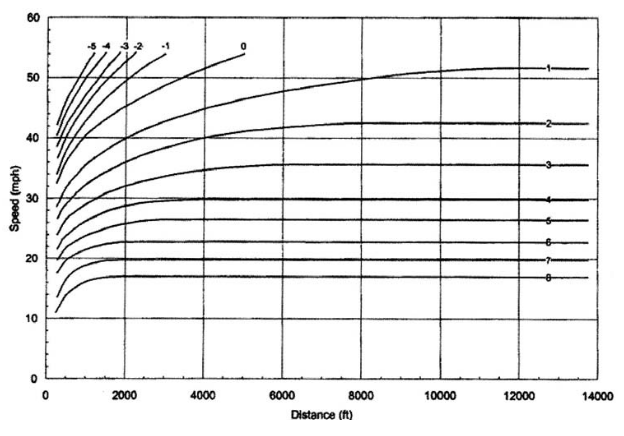
\includegraphics{gfx/fig8.png}
\emph{Fig: Speed-Distance Curves for Acceleration of a Typical Heavy Truck of 120 kg/kw [200 lb/hp] on Upgrades and Downgrades}
\paragraph{Rolling Resistance}
There are forces within the vehicle itself that offer resistance to motion. These forces are due mainly to frictional effect on moving parts of the vehicle, but they also include the frictional slip between the pavement surface and the tires. The sum effect of these forces on motion is known as rolling resistance. The rolling resistance depends on the speed of the vehicle and the type of pavement. Rolling forces are relatively lower on smooth pavements than on rough pavements.\\\\
\par
The rolling resistance force for passenger cars on a smooth pavement can be determined from the relation
\begin{equation}
	R_r = (C_{rs} + 2.15C_{rv} u^2)W
\end{equation}
Where,\\
\hspace*{10mm}$R_r$ = rolling resistance force (lb)\\
\hspace*{10mm}$C_{rs}$ = constant (typically 0.012 for passenger cars)\\
\hspace*{10mm}$C_{rv}$ = constant (typically $0.65 * 10^{-6}$ sec2/ft2 for passenger cars)\\
\hspace*{10mm}$u$ = vehicle speed (mi/h)\\
\hspace*{10mm}$W$ = gross vehicle weight (lb)\\\\
\begin{equation}
	R_r = ( C_{rs} + 0.0772 \times C_{rv} \times u^2)W
\end{equation}
Where,\\
\hspace*{10mm}$R_r$ = rolling resistance force (N)\\
\hspace*{10mm}$C_{rs}$ = constant (typically 0.012 for passenger cars)\\
\hspace*{10mm}$C_{rv}$ = constant (typically $6.99 \times 10^{-6}$ $ sec^2/m^2 $ for passenger cars)\\
\hspace*{10mm}$u$ = vehicle speed (Km/h)\\
\hspace*{10mm}$W$ = gross vehicle weight (N)\\\\
For trucks, the rolling resistance can be obtained from
\begin{equation}
	R_r = (C_a+1.47C_b u)W
\end{equation}
Where,\\
\hspace*{10mm}$R_r$ = rolling resistance force (lb)\\
\hspace*{10mm}$C_a$ = constant (typically 0.2445 for trucks)\\
\hspace*{10mm}$C_b$ = constant (typically 0.00044 sec/ft for trucks)\\
\hspace*{10mm}$u$ = vehicle speed (mi/h)\\
\hspace*{10mm}$W$ = gross vehicle weight (lb)
\begin{equation}
	R_r = (C_a + 0.278 \times C_b \times u)\times W
\end{equation}
Where,\\
\hspace*{10mm}$R_r$ = rolling resistance force (N)\\
\hspace*{10mm}$C_a$ = constant (typically 0.2445 for trucks)\\
\hspace*{10mm}$C_b$ = constant (typically $1.44 \times 10^{-3}$ sec/m  for trucks)\\
\hspace*{10mm}$u$ = vehicle speed (Km/h)\\
\hspace*{10mm}$W$ = gross vehicle weight (N)\\\\
The surface condition of the pavement has a significant effect on the rolling resistance. For example, at a speed of 50 mi/h on a badly broken and patched asphalt surface, the rolling resistance is 51 lb/ton of weight, whereas at the same speed on a loose sand surface, the rolling resistance is 76 lb/ton of weight.
\paragraph{Curve Resistance}
When a passenger car is maneuvered to take a curve, external forces act on the front wheels of the vehicle. These forces have components that have a retarding effect on the forward motion of the vehicle. The sum effect of these components constitutes the curve resistance. This resistance depends on the radius of the curve, the gross weight of the vehicle, and the velocity at which the vehicle is moving. It can be determined as
\begin{equation}
	R_c = 0.5 \frac{(2.15 u^2 W)}{gR}
\end{equation}
Where,\\
\hspace*{10mm}$R_c$ = curve resistance (lb)\\
\hspace*{10mm}$u$ = vehicle speed (mi/h)\\
\hspace*{10mm}$W$ = gross vehicle weight (lb)\\
\hspace*{10mm}$g$ = acceleration due to gravity ($ft/sec^2$)\\
\hspace*{10mm}$R$ = radius of curvature (ft)
\begin{equation}
	R_c = 0.5 \times \frac{0.0772 \times u^2 \times W}{g \times R}
\end{equation}
Where,\\
\hspace*{10mm}$R_c$ = curve resistance (N)\\
\hspace*{10mm}$u$ = vehicle speed (Km/h)\\
\hspace*{10mm}$W$ = gross vehicle weight (N)\\
\hspace*{10mm}$g$ = acceleration due to gravity ($m/sec^2$)\\
\hspace*{10mm}$R$ = radius of curvature ($ m $)
\paragraph{Power Requirements}
Power is the rate at which work is done. It is usually expressed in horsepower (a U.S. unit of measure), where 1 horsepower is 550 lb-ft /sec. The performance capability of a vehicle is measured in terms of the horsepower the engine can produce to overcome air, grade, curve, and friction resistance forces and put the vehicle in motion. Figure below shows how these forces act on the moving vehicle.\\
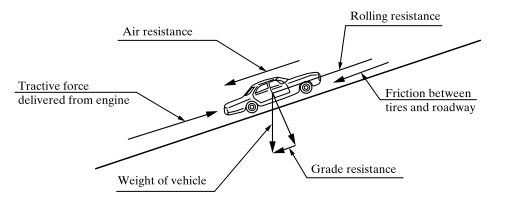
\includegraphics[scale=0.9]{gfx/fig9.png}\\
The power delivered by the engine is
\begin{equation}
	P = \frac{1.47Ru}{550}
\end{equation}
Where,\\
\hspace*{10mm}$P$ = horsepower delivered (hp)\\
\hspace*{10mm}$R$ = sum of resistance to motion (lb)\\
\hspace*{10mm}$u$ = speed of vehicle (mi/h)
\begin{equation}
	P = \frac{0.278 \times F \times u}{76.04}
\end{equation}
Where,\\
\hspace*{10mm}$P$ = horsepower delivered (hp)\\
\hspace*{10mm}$R$ = sum of resistance to motion (Kg)\\
\hspace*{10mm}$u$ = speed of vehicle (Km/h)\\\\
\emph{Numerical Example:}\\
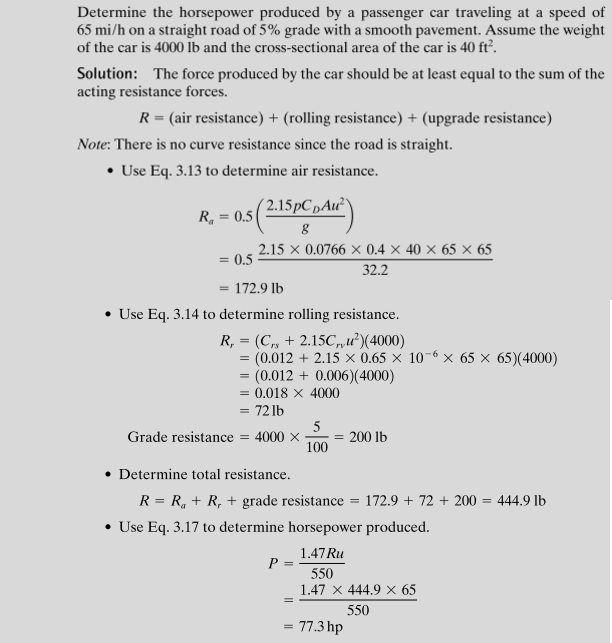
\includegraphics[scale=0.5]{gfx/fig10.png}\\
\subsection{Pedestrian Characteristics}
Pedestrian characteristics relevant to traffic and highway engineering practice include those of the driver, discussed in the preceding sections. In addition, other pedestrian characteristics may influence the design and location of pedestrian control devices. Such control devices include special pedestrian signals, safety zones and islands at intersections, pedestrian underpasses, elevated walkways, and crosswalks. Apart from visual and hearing characteristics, walking characteristics play a major part in the design of some of these controls. For example, the design of an all-red phase, which permits pedestrians to cross an intersection with heavy traffic, requires knowledge of the walking speeds of pedestrians. Observations of pedestrian movements have indicated that walking speeds vary between 3.0 and 8.0 ft /sec. Significant differences have also been observed between male and female walking speeds. At intersections, the mean male walking speed has been determined to be 4.93 ft /sec, and for females, 4.63 ft /sec. A more conservative value of 4.0 ft /sec is normally used for design purposes. However, Rouphail and others have shown that the average walking speed depends on the population of elderly pedestrians. For example, the average walking speed is 4.0 ft /sec when the percentage of elderly pedestrians is 20 percent or lower, but reduces to 3.0 ft /sec when the percentage of elderly pedestrians is higher than 20 percent. This factor therefore should be taken into consideration for the design of intersection pedestrian signals at locations where a high number of older pedestrians is expected. Consideration also should be given to the characteristics of handicapped pedestrians, such as the blind. Studies have shown that accidents involving blind pedestrians can be reduced by installing special signals. The blind pedestrian can turn the signal to a red phase by using a special key, which also rings a bell, indicating to the pedestrian that it is safe to cross. Ramps are also now being provided at intersection curbs to facilitate the crossing of the intersection by the occupant of a wheelchair. Also, consideration should be given to the relatively lower average walking speed of the handicapped pedestrian, which can vary from a low of 1.97 ft /sec to 3.66 ft /sec.\\
%
\subsection{Road Characteristics}
The characteristics of the highway discussed in this section are related to stopping and passing because these have a more direct relationship to the characteristics of the driver and the vehicle discussed earlier.
\subsubsection{Sight Distance}
Sight distance is the length of the roadway a driver can see ahead at any particular time. The sight distance available at each point of the highway must be such that, when a driver is traveling at the highway’s design speed, adequate time is given after an object is observed in the vehicle’s path to make the necessary evasive maneuvers without colliding with the object. The two types of sight distance are (1) stopping sight distance and (2) passing sight distance.
\paragraph{\emph{1. Stopping Sight Distance}}
The stopping sight distance (SSD), for design purposes, is usually taken as the minimum sight distance required for a driver to stop a vehicle after seeing an object in the vehicle’s path without hitting that object. This distance is the sum of the distance traveled during perception-reaction time and the distance traveled during braking. The SSD for a vehicle traveling at u mi/h is
\begin{equation}
	SSD = 1.47ut + \frac{u^2}{30\left(\frac{a}{g} \pm G \right)}
\end{equation}
Where,\\
\hspace*{10mm}$u$ = speed of the vehicle when brakes are appled\\
\hspace*{10mm}$t$ = distance travelled between perception-reaction time\\
\hspace*{10mm}$g$ = acceleration due to gravity\\
\hspace*{10mm}$a$ = acceleration of the vehicle\\
\hspace*{10mm}$G$ = $\tan \gamma$ (\% Grade/100)\\\\
\paragraph{\emph{2. Passing Sight Distance}}
The passing sight distance is the minimum sight distance required on a two-lane, twoway highway that will permit a driver to complete a passing maneuver without colliding with an opposing vehicle and without cutting off the passed vehicle. The passing sight distance will also allow the driver to successfully abort the passing maneuver (that is, return to the right lane behind the vehicle being passed) if he or she so desires. In determining minimum passing sight distances for design purposes, only single passes (that is, a single vehicle passing a single vehicle) are considered. Although it is possible for multiple passing maneuvers to occur (that is, more than one vehicle pass or are passed in one maneuver), it is not practical for minimum design criteria to be based on them.\\\\
\emph{Numerical Example:}\\
Drivers with an average 20/40 vision travel at 55 mph in the curb lane of a freeway, where the exit ramps are designed for 25 mph. What should be the minimum distance of the sign with 6 inch letters placed ahead of the exit? (perception-reaction time = 2.5 sec, deceleration rate = 5 ft/s2 , drivers with 20/20 vision can read the sign at 60 ft per inch of letter height)\\
\emph{Solution}:\\\\
initial velocity ($ u $) = 55 mph; final velocity ($ v $) = 25 mph ; perception reaction time ($ t $) = 2.5 sec; 	deceleration rate ($ a $) = 5 ft/s2 \\\\
now,\\
Decelerating distance ($ d_1 $) = $ \frac{u^2 - v^2}{2 \times a} $ = $ \frac{55^2 - 25^2}{2 \times 5} \times \frac{5280}{3600}^2 $ = 516 ft\\\\
Also,\\
distance for a 20/20 vision to read the sign ($ D_{normal} $) = 60 $ \times $ 6 = 360 ft\\
visual acuity ($ X $) = 20/40 = 0.5\\\\
$ \therefore D_{sight} $ =$ D_{normal} \times X $ = $ 360 \times 0.5 $ = 180 ft\\\\
then,\\
Then,
distance required to react the stimulus ($ d_2 $) = u $ \times $ t = 55 $ \times $ (2.5/3600) = 202 ft\\\\
Now,\\
the minimum distance where the sign should placed ahead of the exit ramp($ d $) = $ d_1 + d_2 - d_{sight} $= 516 + 202 – 180 = 538 ft\\
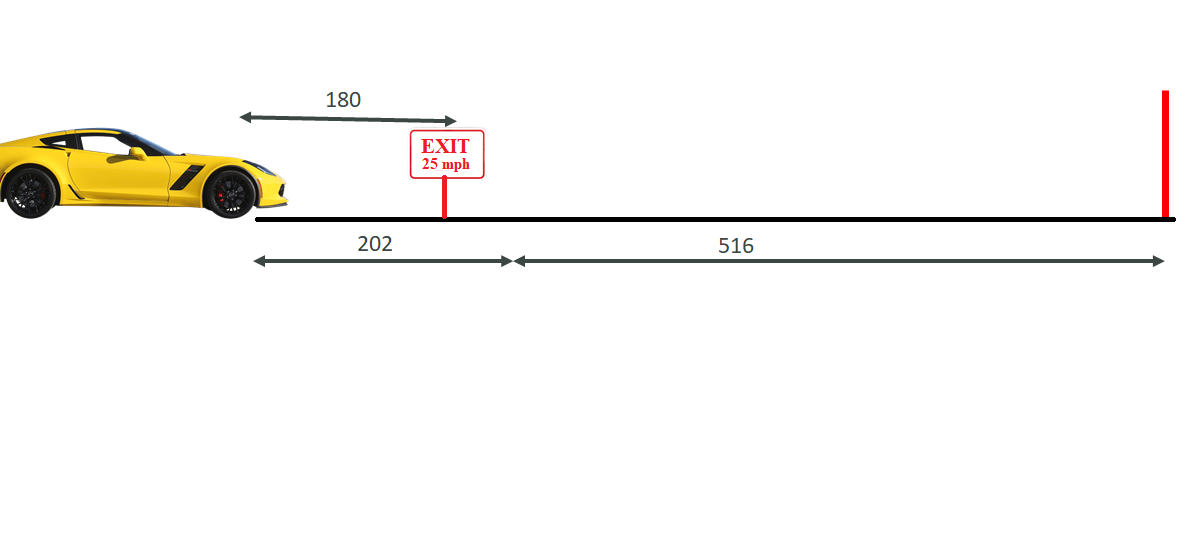
\includegraphics[scale=0.3]{gfx/visualAquityNum.png}
\newpage
\section{Review Problems}
\begin{enumerate}
	\item  Explain Perception-Reaction process with a relevant example.
	\item  Define Visual Acuity and 20/20 vision. Derive the expression for visual angle.
	\item  Derive the mathematical expression for kinematic characteristics of a vehicle.
	\item Determine the difference in air resistance between a passenger car and a single-unit truck if both vehicles are traveling at a speed of 96.5 km/h. Assume that the frontal cross-sectional area of the passenger car is 2.79 $ m^2 $ and that for the truck is 10.70 $ m^2 $. [1903.6 N]
	\item Determine the rolling resistance on a passenger car that is traveling at 105 km/h if the weight of the car is 9000 N. [161.1 N]
	\item A single-unit three-axle truck traveling on an interstate highway at a speed of 88.5 km/h approaches a horizontal curve with a radius of 274.25 m. Determine the curve resistance that acts on the truck as it traverses the curve if the weight on each axle is 22675 N. [7644.1 N]
	\item A 13600 N passenger car is traveling at 88.5 km/h on a flat section of road with a horizontal curve of 300 m radius. If the cross-sectional area of the vehicle is 2.7 $ m^2 $, determine the horsepower required to overcome the resistance on the vehicle. [65.56 hp]
	\item Two passenger cars are traveling at 88.5 km/h.The weight of car A is 9000 N, and that of car B is 18000 N.The cross-sectional area for car A is 3.15 $ m^2 $, and that of car B is 3.6 $ m^2 $. Determine the maximum grade on which passenger car A can travel without its total resistance exceeding that of car B traveling on a straight and level section of road.[ 2.36 \%]
	\item A passenger car being driven on a flat and straight section of a highway at a speed of 105 km/h reaches a curved section of the highway with a grade of 5\% and a radius of 450 m. Determine:
		\begin{enumerate}
			\item The additional force that will be required to maintain the original speed of 105 km/h [1302.63 N]
			\item The percentage increase in the total force to maintain the original speed of 105 km/h [59.3 \%]
		\end{enumerate}
	Assume that the weight of the car is 907 kg, the cross-sectional area is 3.15 $ m^2 $, and the car is being driven at sea level.
	\item A truck and a passenger car traveling on a section of highway at a speed of 80 km/h enter a short curved section of the road with a grade of 5\% and a radius of 270 m. Determine the ratio of the additional force required by the truck to that required by the car for both vehicles to maintain their original speed of 80 km/h. Assume the weight of the car is 11250 N and that of the truck 54000 N. [5 : 1]
\end{enumerate}




